\def\mytitle{ASSIGNMENT-1}
\def\myauthor{D. Siva Krishna}
\def\contact{r170582@rguktrkv.ac.in}
\def\mymodule{Future Wireless Communications (FWC)}
\documentclass[10pt, a4paper]{article}
\usepackage[a4paper,outer=1.5cm,inner=1.5cm,top=1.75cm,bottom=1.5cm]{geometry}
\twocolumn
\usepackage{graphicx}
\graphicspath{{./images/}}
\usepackage[colorlinks,linkcolor={black},citecolor={blue!80!black},urlcolor={blue!80!black}]{hyperref}
\usepackage[parfill]{parskip}
\usepackage{lmodern}
\usepackage{tikz}

\usepackage{karnaugh-map}

\usepackage{tabularx}
%\documentclass{article}
%\documentclass[tikz, border=2mm]{standalone}
%\usepackage{tikz}
%\usepackage{circuitikz}
\usetikzlibrary{calc}

\renewcommand*\familydefault{\sfdefault}
\usepackage{watermark}
\usepackage{lipsum}
\usepackage{xcolor}
\usepackage{listings}
\usepackage{float}
\usepackage{titlesec}

\titlespacing{\subsection}{1pt}{\parskip}{3pt}
\titlespacing{\subsubsection}{0pt}{\parskip}{-\parskip}
\titlespacing{\paragraph}{0pt}{\parskip}{\parskip}
\newcommand{\figuremacro}[5]{
    \begin{figure}[#1]
        \centering
        \includegraphics[width=#5\columnwidth]{#2}
        \caption[#3]{\textbf{#3}#4}
        \label{fig:#2}
    \end{figure}
}

\lstset{
frame=single, 
breaklines=true,
columns=fullflexible
}

%\thiswatermark{\centering \put(400,-128.0){\includegraphics[scale=0.3]{logo}} }
\title{\mytitle}
\author{\myauthor\hspace{1em}\\\contact\\IITH\hspace{0.5em}-\hspace{0.6em}\mymodule}
\date{19-09-2022}
\begin{document}
  \maketitle
  \tableofcontents
  \begin{abstract}
      This manual explains about 4-bit shift register through 7474 IC in Arduino  :
%\figuremacro{h}{diag}{}{}{0.9}
  \end{abstract}

  
\section{Introduction}
    \subsection{7474 IC:}
This IC contains 2 D-flip flops.\\
For this section total of 4 flip-flops(2 ICs) are required since we need to design a 4-bit shift register.

\subsection{Arduino:}
    In Arduino Uno we generate the clock pulse which is given to the each and every flip-flop by default.\\
    We take 5 volts and Ground as the supply to the bread board from the Arduino board.


  \section{Components}
  \begin{tabularx}{0.4\textwidth} { 
  | >{\centering\arraybackslash}X 
  | >{\centering\arraybackslash}X 
  | >{\centering\arraybackslash}X
  | >{\centering\arraybackslash}X | }
\hline
 \textbf{Component}& \textbf{Values} & \textbf{Quantity}\\
\hline
Arduino & UNO & 1 \\  
\hline
JumperWires& M-M & 20 \\ 
\hline
Breadboard &  & 1 \\
\hline
IC & 7447 &2 \\
\hline
\end{tabularx}

\section{PIN Diagram}
\begin{center}
    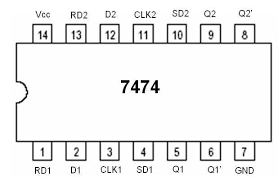
\includegraphics{7474.png}
\end{center}


\begin{center}
Figure.a
\end{center}

\section{Truth Table}
  \begin{tabularx}{0.46\textwidth} { 
  | >{\centering\arraybackslash}X 
  | >{\centering\arraybackslash}X 
  | >{\centering\arraybackslash}X
  | >{\centering\arraybackslash}X 
  | >{\centering\arraybackslash}X 
  | >{\centering\arraybackslash}X 
  | >{\centering\arraybackslash}X 
  | >{\centering\arraybackslash}X 
  | >{\centering\arraybackslash}X 
  | >{\centering\arraybackslash}X | }


\hline
\textbf{D1} & \textbf{Q1=D2} & \textbf{Q2=D3} & \textbf{Q3=D4}  & \textbf{Q4}\\
\hline
0 & 0 & 0 & 0 & 0 \\  
\hline
1 & 1 & 0 & 0 & 0 \\ 
\hline
1 & 1 & 1 & 0 & 0 \\
\hline
0 & 0 & 1 & 1 & 0 \\
\hline
1 & 1 & 0 & 1 & 1 \\  
\hline
0 & 0 & 1 & 0 & 1\\ 
\hline
0 & 0 & 0 & 1 & 0 \\
\hline
0 & 0 & 0 & 0 & 1 \\
\hline
0 & 0 & 0 & 0 & 0 \\
\hline
\end{tabularx}
\begin{center}
 Truth table for 1011
\end{center}

\section{Circuit Diagram}
\begin{figure}
\centering
    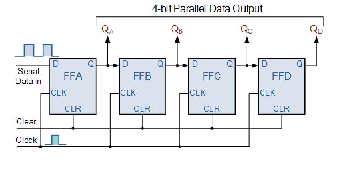
\includegraphics[width=4in]{shift-reg.png}
\end{figure}

 \paragraph {shift-register}It has 4 D-flip flops.\\
    It takes 1 input that is D1.\\
    It has 4 outputs i.e Q1, Q2, Q3 and Q4.\\
    By default it takes the input from LSB to MSB.\\

    
\section{Implementation}
  \begin{tabularx}{0.96\textwidth} { 
  | >{\centering\arraybackslash}X 
  | >{\centering\arraybackslash}X 
  | >{\centering\arraybackslash}X
  | >{\centering\arraybackslash}X 
  | >{\centering\arraybackslash}X 
  | >{\centering\arraybackslash}X 
  | >{\centering\arraybackslash}X 
  | >{\centering\arraybackslash}X 
  | >{\centering\arraybackslash}X
  | >{\centering\arraybackslash}X
  | >{\centering\arraybackslash}X
  | >{\centering\arraybackslash}X
  | >{\centering\arraybackslash}X
  | >{\centering\arraybackslash}X
  | >{\centering\arraybackslash}X 
  | >{\centering\arraybackslash}X | }


\hline
\textbf{Ard} & \textbf{D13} & \textbf{D13} &  &  &  & \textbf{Vcc} & \textbf{Vcc} & \textbf{Vcc} & \textbf{Vcc} & \textbf{Vcc} & \textbf{Gnd} &  &  &  & \\  
\hline
\textbf{7474} & 3 & 11 & 5-12 & 9 &  & 1 & 4 & 10 & 13 & 14 & 7 & 5 & 9 &  &  \\
\hline
\textbf{7474} & 3 & 11 &  & 2 & 5-12 & 1 & 4 & 10 & 13 & 14 & 7 &  &  & 5 & 9  \\
\hline
\textbf{LED} &  &  &  &  &  &  &  &  &  &  &  & led1 & led2 & led3 & led4  \\
\hline
\end{tabularx}

\begin{center}
    Connections
\end{center}

    \paragraph{Problem-1}
    
    1. Connect the circuit as per the above table.\\
    2. Execute the circuit using the below code.\\
\begin{tabularx}{0.46\textwidth} { 
  | >{\centering\arraybackslash}X |}
  \hline
  https://github.com/siva-krishna-IITH-2022/fwc-assign/Assignment-1/AVR GCC/codes\\
  \hline
\end{tabularx}
   \paragraph{Problem-2}
1. Same circuit can be implemented by connecting a,b,c and d terminals of seven segment display to the Q1, Q2, Q3 AND Q4 respectively instead of using 4 LEDs.\\
2. Execute the circuit using the above code.\\


\bibliographystyle{ieeetr}
\end{document}